\documentclass[10pt,twocolumn,letterpaper]{article}

\usepackage{cvpr}
\usepackage{times}
\usepackage{epsfig}
\usepackage{graphicx}
\usepackage{amsmath}
\usepackage{amssymb}
\usepackage{listings}
\usepackage{lipsum}

\lstset{breaklines=true}
% Include other packages here, before hyperref.

% If you comment hyperref and then uncomment it, you should delete
% egpaper.aux before re-running latex.  (Or just hit 'q' on the first latex
% run, let it finish, and you should be clear).

\usepackage[pagebackref=true,breaklinks=true,letterpaper=true,colorlinks,bookmarks=true,bookmarksnumbered=true,hypertexnames=false,linkbordercolor={0 0 1}]{hyperref}
% Include other packages here, before hyperref.

% If you comment hyperref and then uncomment it, you should delete
% egpaper.aux before re-running latex.  (Or just hit 'q' on the first latex
% run, let it finish, and you should be clear).
%\usepackage[pagebackref=true,breaklinks=true,letterpaper=true,colorlinks,bookmarks=false]{hyperref}

\cvprfinalcopy % *** Uncomment this line for the final submission

\def\cvprPaperID{****} % *** Enter the CVPR Paper ID here
\def\httilde{\mbox{\tt\raisebox{-.5ex}{\symbol{126}}}}

% Pages are numbered in submission mode, and unnumbered in camera-ready
\ifcvprfinal\pagestyle{empty}\fi
%\setcounter{page}{1}
\begin{document}

%%%%%%%%% TITLE
\title{Your Final Project Title}

\author{Team Members\\
Department Names\\
UNiversity of Wisconsin-Madison\\
{\tt\small authors@wisc.edu}
% For a paper whose authors are all at the same institution,
% omit the following lines up until the closing ``}''.
% Additional authors and addresses can be added with ``\and'',
% just like the second author.
% To save space, use either the email address or home page, not both
\and
Team Members\\
Department Names\\
UNiversity of Wisconsin-Madison\\
{\tt\small authors@wisc.edu}
}

\maketitle
%\thispagestyle{empty}


%%%%%%%%% BODY TEXT
\section{Optimal Seam Search}

After we warped the two images, we need to find an optimal seam along which the area extracted from the source image can be determined. There are three main concerns for the search. First, we want to avoid the the important features in face, such as eye, month, nose and so on. Second, the pixels on the boundary of the extracted area should be similar between the two images so that it will be more natural when we composite them together. Third, we want to reduce the computation complexity.

Our approach is based on Kwatra et al's work \cite{kwatra2003graphcut}. The algorithm works by formulating the image as a connected graph with edge weights based on the difference between neighboring pixels. This graph is then treated as a max-flow/min-cut problem where the sources are any pixels to be taken only from the first image and the sinks are any pixels to be taken only from the second image.

\begin{figure}[hb]
  \centering
  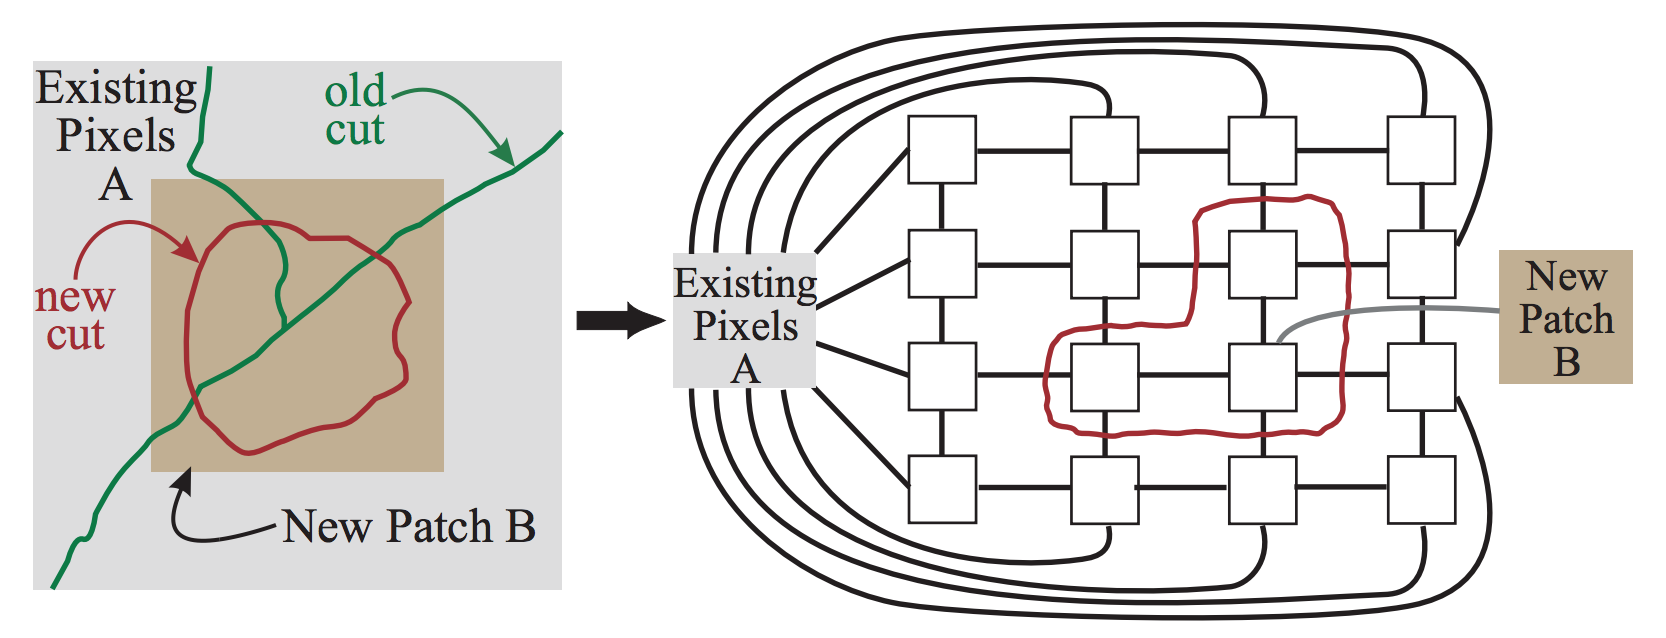
\includegraphics[width=0.4\textwidth]{graph_image.png}
  \caption{Graph representation of image, from \cite{kwatra2003graphcut}}\label{graph}
\end{figure}

As the figure \ref{graph} shows, in our project, the pixels in patch A must from our target image while the pixels in patch B must from source image. The goal is to find the optimal cut between patch A and patch B. We represent the image graph as an adjacency matrix while each entry in the adjacency matrix can be the flow. We use the sum of absolute difference between the source image and the target image plus the sum of absolute difference of the source image and the target image at the neighboring pixel.

\begin{equation}
M(c,n,S,T) = \Vert S(c) - T(c) \Vert_1 + \Vert S(n) - T(n) \Vert_1
\end{equation}

where $c$ is the current pixel, $n$ is the neighbor pixel, $S$ is the source image and $T$ is the target image. The $L1$ norm is the sum of absolute difference of these two pixels in three channels. Note that the weight between the pixels in patch A and its neighbors must be infinity. This is same for patch B.

In our implementation, we first define the permissible path region by generating two masks based on the landmarks generated from the first step, shown in \ref{seam-mask}. The permissible path region is the area we want to find the optimal seam. All the pixels which are outside the right larger mask must from target image, i.e. patch B, and all the pixels inside the left smaller mask must from source image, i.e. patch A. Therefore, the permissible path region is the area which is inside the larger mask but outside the smaller mask. As the forehead region of a face is usually more flat than the other regions. A good permissible region is crucial to the following steps. First, the permissible path should not be too strict, then it's highly possible that we cannot find the optimal seam within the strict area. Second, the larger the permissible path region is, the higher computation complexity will be. Thus, when constructing the two masks, a convex hull is constructed by the landmarks. Then we split the face into two regions: the forehead region and the bottom region. For the forehead region, as the convex hull is right above the eyes while the forehead region is relatively flat, the mask is eroded so that the permissible path region will cover larger area. For the bottom region, because the convex hull is almost the boundary of the face, it is not reasonable to extend the permissible path outside the face, the mask is dilated. After generating two masks for each region via erosion and dilation, we stitch them together to get the final permissible path region.

For the construction of the adjacency matrix, we extend the patch A and patch B by including all the pixels which are immediate neighbors. In other words, if the neighbor of a pixel is in patch A or B, then the weight between them is also infinite. If the weight between two pixels is not infinite, then these two pixels must be 1) not in patch A and patch B and 2) their neighbors are also not in patch A and patch B.

\begin{figure}[hb]
  \centering
  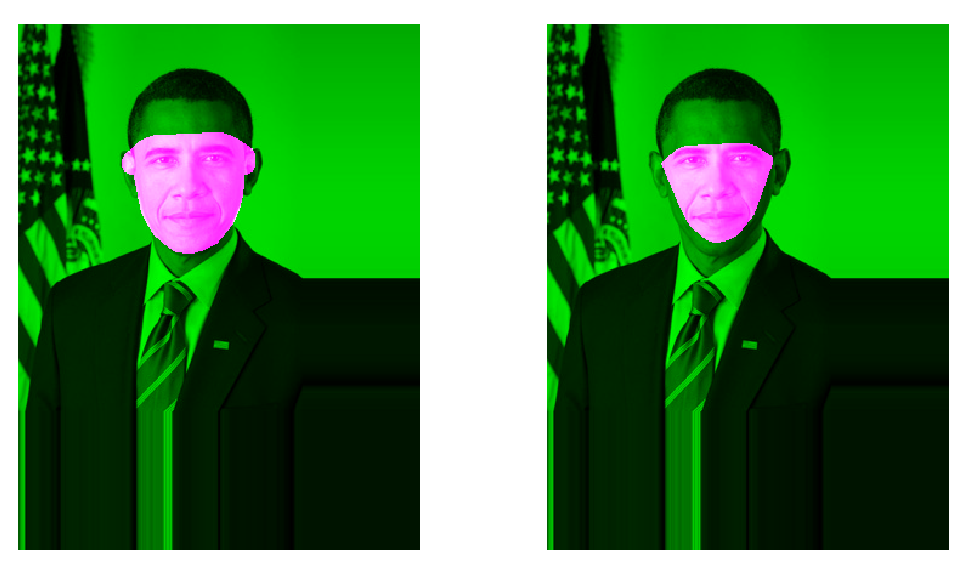
\includegraphics[width=0.4\textwidth]{seam_mask.eps}
  \caption{Mask for optimal seam search}\label{seam-mask}
\end{figure}

The result is shown in Fig.\ref{seam-result}. The pink area is the permissible path region and the red circle in the left figure is the result.

\begin{figure}[hb]
  \centering
  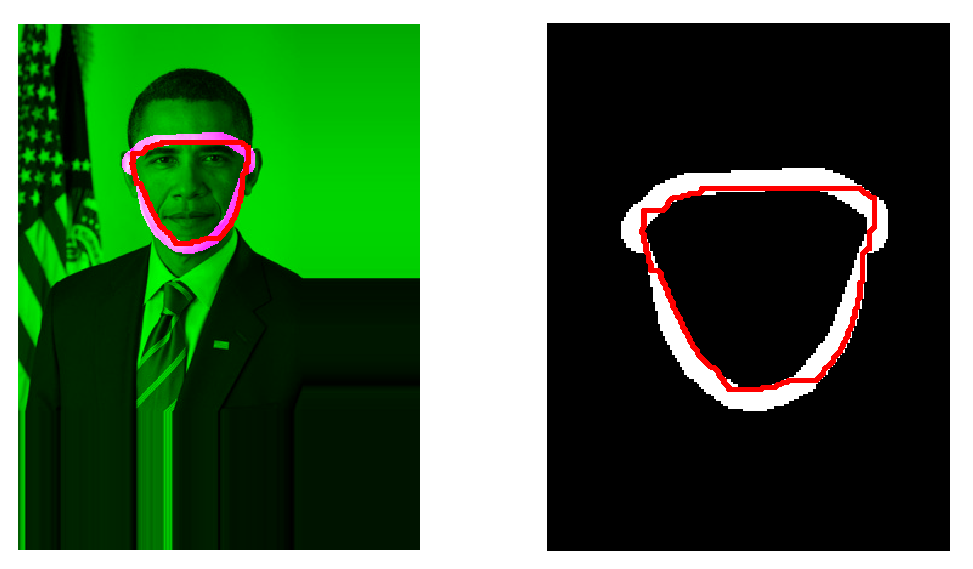
\includegraphics[width=0.4\textwidth]{seam_result.eps}
  \caption{Result for optimal seam search}\label{seam-result}
\end{figure}

\begin{lstlisting}
%mask_dst is initialized as the convex hull of the landmarks in target image
top_mask = mask_dst;
bottom_mask = mask_dst;
%split the mask into forehead region and bottome region
[v, indx] = max(mask_dst,[],1);
bd = indx(find(v==1,1));
top_mask(bd+1:end,:) = 0;
bottom_mask(1:bd,:) = 0;
%dilate for the forehead region
SE_disk = strel('disk',10,6);
top_mask_outer = imdilate(top_mask, SE_disk);
top_mask_inner = top_mask;
%erode for the bottom region
bottom_mask_outer = bottom_mask;
SE_disk = strel('disk',10,6);
bottom_mask_inner = imerode(bottom_mask, SE_disk);
%stitch the masks for the two regions together
mask_outer = logical(top_mask_outer + bottom_mask_outer);
mask_inner = bwconvhull(logical(top_mask_inner + bottom_mask_inner));
%mask is the area where we want to get the optimal seam
mask = mask_outer - mask_inner;
\end{lstlisting}

\section{Face Blending}

The optimal seam shows us what is the best area which should be extract from the source image. If we simply cut that area from the source image and paste it to the target image, the result will not be satisfiable, as the left image shown in Fig\ref{blending}. The problem is the color of these two images are very different from each other. Therefore, we can see the color change abruptly around the boundary. In order to avoid the abrupt color changes, we use Poisson blending approach.

\begin{figure}[hb]
  \centering
  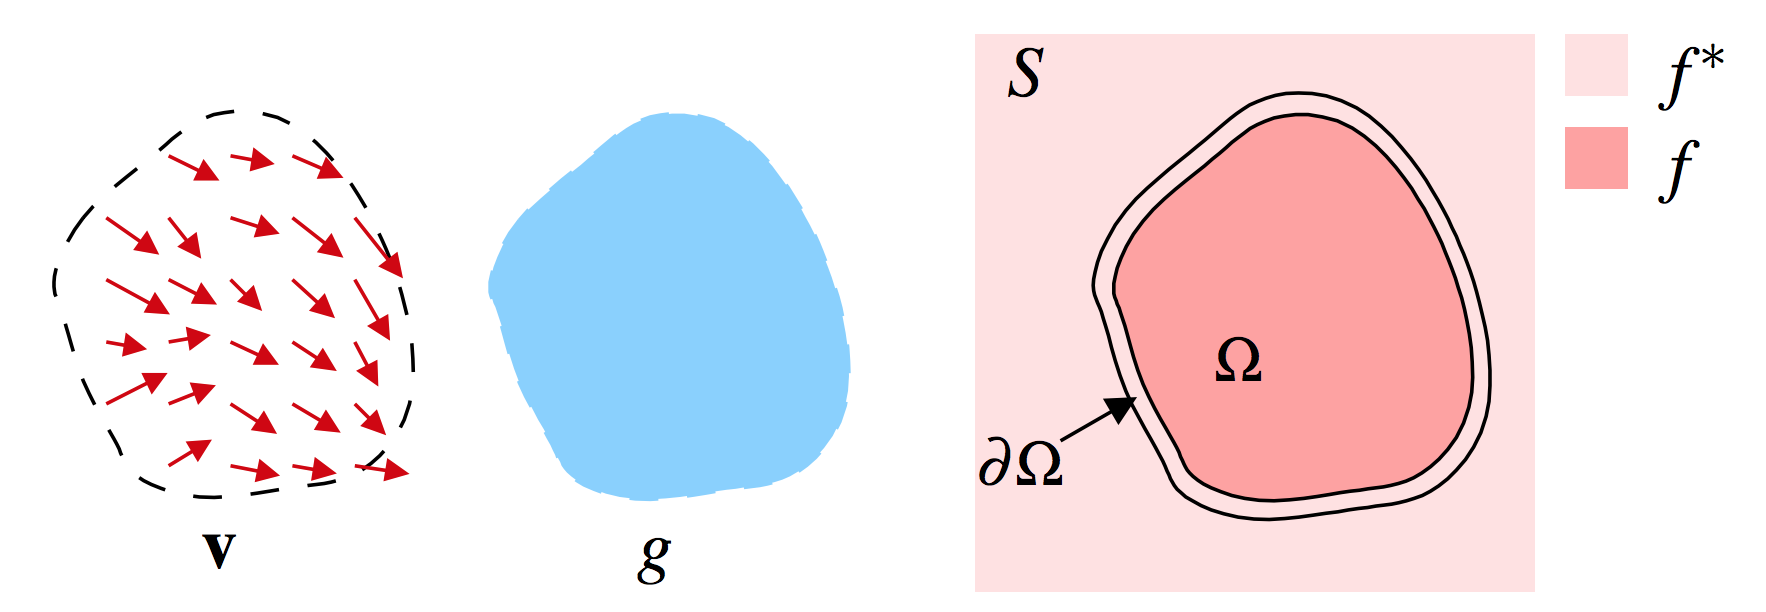
\includegraphics[width=0.4\textwidth]{poisson_blending_alg.png}
  \caption{Poisson blending notation, \cite{perez2003poisson} }\label{blending_alg}
\end{figure}

Poisson blending is one of gradient domain image processing methods. As Fig.\ref{blending_alg} shown, $v$ is gradient of a region in an image, $g$ is selected region of source, $f^*$ is a known functions that exist in domain $S$, $f$ is an unknown functions that exist in domain $\Omega$, $\Omega$ is a region $g$ that is now placed on domain $S$ (target background), $\partial{\Omega}$ is boundaries between the source and target regions. The goal is given $v$, find the value of $f$ in the unknown region that optimize

\begin{eqnarray}
min_{f} & \iint_{\Omega} \vert \nabla f -v \vert^2  \\
\mbox{subject to} & f \mid_{\partial{\Omega}} = f^* \mid_{\partial{\Omega}}
\end{eqnarray}
where $\nabla = [\frac{\partial{}}{\partial{x}}, \frac{\partial{}}{\partial{y}}]$ is the gradient vector. Its solution is the unique solution of the following Poisson equation with Dirichlet boundary conditions:

\begin{eqnarray}
& \Delta f = \mbox{div }v \quad \mbox{over } \Omega \\
\mbox{subject to} & f \mid_{\partial{\Omega}} = f^* \mid_{\partial{\Omega}}
\end{eqnarray}
where $\mbox{div} v = \frac{\partial{u}}{\partial{x}} + \frac{\partial{v}}{\partial{x}}$ is the divergence of $v = (u,v)$, and $\Delta$ is the Laplacian operator as follows:

\begin{table}[h]
\centering
\begin{tabular}{|l|l|l|}
\hline
 0 & -1 & 0 \\ \hline
 -1 & 4 & -1  \\ \hline
 0 & -1 & 0  \\ \hline
\end{tabular}
\end{table}

This is the fundamental machinery of Poisson editing of color images: three Poisson equations of the above equation are solved independently in the three color channels of the chosen color space.

\begin{figure}[hb]
  \centering
  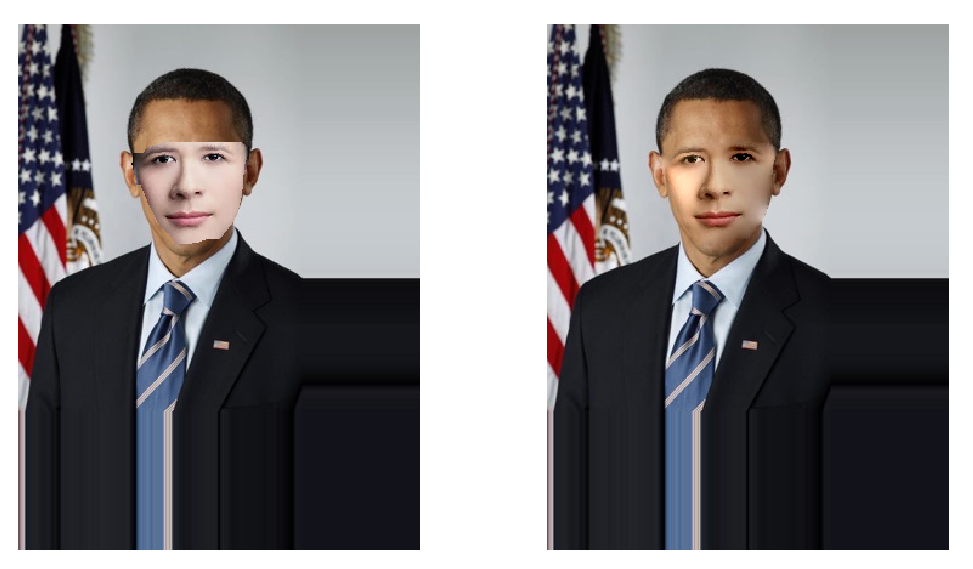
\includegraphics[width=0.4\textwidth]{possion_blending_result.eps}
  \caption{Poisson blending}\label{blending}
\end{figure}


{\small
\bibliographystyle{ieee}
\bibliography{report}
}


\end{document}
